\chapter{Bilan}

\section{Problèmes rencontrées}

\flushleft La plupart des problèmes étaient liés au MinMax et surtout à la façon de gérer plusieurs objet Board.
En effet, pendant le fonction MinMax, énormément de coups sont joués sur des Boards différentes.
Nous avons donc finit par réussir en comprenant mieux comment fonctionne les objets.
\\
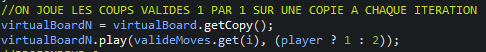
\includegraphics[width=0.60\textwidth]{./VIRTUALBOARD}
\\
Alphabeta ne fut pas implémenté probablement à cause de problème de référencement et de la classe
AlphaBeta. Le problème est peut être aussi le même que lors des premières tentatives d'implémentation
de MinMax. MinMax était incompatible avec notre jeu, il est possible qu'ici AlphaBeta soit incompatible
avec notre version actuelle de MinMax.\\


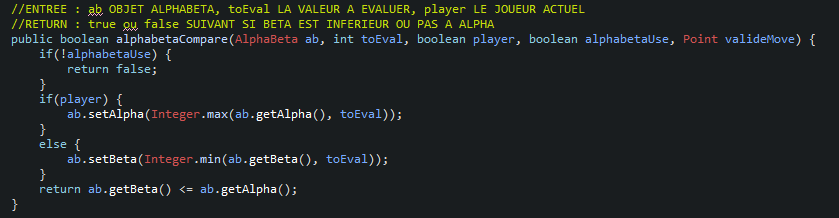
\includegraphics[width=0.60\textwidth]{./ALPHABETA}
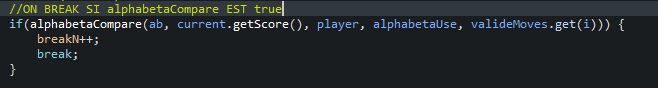
\includegraphics[width=0.60\textwidth]{./ALPHABETA2}

Nous n'avons pas réussit a tracer la courbe nodesperdeep4 car les méthodes pour dessiner la courbe
n'acceptaient pas les BigInteger en paramètre, et le nombre de nœuds total lors d'une partie
jouée par un MinMax4 est supérieur a 2\up{15}. Nous étions donc obligé de récupérer ce nombre dans une
variable BigInteger.
\\
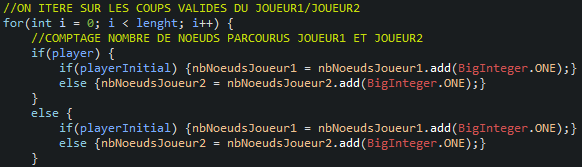
\includegraphics[width=0.60\textwidth]{./BIGINTEGER}
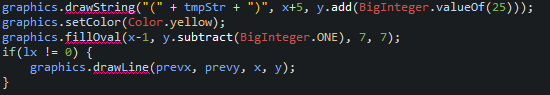
\includegraphics[width=0.60\textwidth]{./BIGINTEGER2}
\\

Le passage de paramètre a Main est différent quand on exécute le programme dans un terminal ou dans
un IDE. Nous avons trouvé comment gérer cela sous Eclipse.
\\
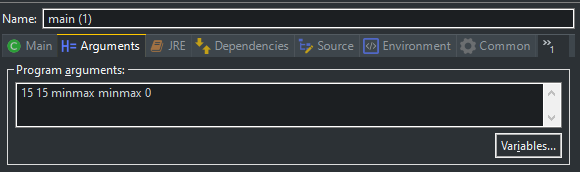
\includegraphics[width=0.60\textwidth]{./MAINPARAM}
\\
\newpage
Enfin, il y avait une redondance du code dans le Main, l'objectif était donc de factoriser le code, pour résoudre ce problème nous avons crée une fonction CurrentPlayer afin de ne pas répéter les opérations du joueur 1 et du joueur 2 

\section{Conclusion}

Ce projet nous a permit de découvrir plusieurs fonctionnalités du langage Java.
Il nous a aussi permit de travailler sur un algorithme très intéressant, et de mieux
comprendre la récursivité ainsi que les structures arborescente.
